\section{Geometry Specification} \label{geometry}\index{Geometry!specification}
The molecular or unit cell geometry is supplied in the data-set as one atom per
line.  \index{Dummy atoms}\index{XX} Sometimes it is useful to have points
within a geometry defined.  These points need not represent atoms.  To allow
for this, users can add entities called ``dummy atoms''.

The format in which the data is supplied is atoms essentially the
``Free-Format''   style of FORTRAN-77.   In  fact, a character input is used in
order to accommodate the  chemical  symbols,  but  the  numeric  data  can
be   regarded   as ``free-format''.\index{Data!free-format}    This  means
that  integers  and  real  numbers  can  be interspersed, and numbers can be
separated by one or more spaces, a tab\index{Data!tabs in} and/or  by  one
comma.  If a number is not specified, its value is set to
zero.\index{Data!commas in}

The geometry can be defined in terms of either internal or Cartesian
coordinates, or a mixture of the two, or it can be in PDB or Gaussian format.

\subsection{Definition of Elements and Isotopes}
Elements are defined in terms  of  their  atomic  numbers  or  their chemical
symbols, case insensitive.\index{Isotopes!specification of}   Thus, chlorine
could be specified as 17, or Cl.   \index{Elements!specification of}

Acceptable symbols for MNDO are\index{MNDO!elements in} given in
Table~\ref{mndoel}.

\begin{table}
\begin{center}
\caption{\label{mndoel} Elements available within MNDO}
\hspace*{-0.3in} \compresstable
\begin{tabular}{lllllllllllllllllll}
\multicolumn{7}{l}{Elements}&&&&&\multicolumn{7}{l}{Dummy atom, sparkles and
 Translation Vector} \\
\hline
   H  \\
  Li &&   & Be& B& C& N& O& F           \\
  Na$^{\dag}$&&   &   &Al&Si& P& S&Cl &&&       &                         \\
   K$^{\dag}$&& & Zn&$ *$&Ge& *& *&Br &&&     XX$^{\ddag}$& Cb& ++&  +& $--$&  $-$& Tv$^+$  \\
  Rb$^{\dag}$&&\ldots&  *&$ *$&Sn& *& *& I &&&     99&102&103&104&105&106&107  \\
  *  &&\ldots& Hg&$ *$&Pb& *&   \\
\hline
\end{tabular}
\end{center}
\dag  These symbols refer to elements which lack a basis set.  \\
\ddag  This is the dummy atom for assisting with geometry specification.  \\
$*$  Element not parameterized.  \\
+  This is the translation vector for use with polymers.  \\
\end{table}

\index{Parameter sets!old}\index{Old parameter sets} Old parameters for some
elements are available.  These are  provided to  allow compatibility with
earlier copies of MOPAC.  To use these older parameters, use a keyword composed
of the chemical symbol followed by the year  of  publication  of  the
parameters.  Keywords currently available: \comp{Si1978}, \comp{S1978}.

Table~\ref{am1el} lists all elements available in AM1.

\begin{table}
\begin{center}
\caption{\label{am1el} Elements available within AM1}
\index{AM1!elements in} \hspace*{-1.3in} \compresstable
\begin{tabular}{llllllllllllllllllllll}
\multicolumn{10}{l}{Elements}&&&&&\multicolumn{7}{l}{Dummy atom,
sparkles and
 Translation Vector} \\
\hline
  H  \\
   * &$*$&    & && &  & B& C& N& O& F           \\
  Na$^{\dag}$&$*$ && & &  &   &Al&Si& P& S&Cl &&&       &
\\
   K$^{\dag}$&$*$&&Fe& &Cu& Zn&$ *$&Ge&As&Se&Br &&&     XX$^{\ddag}$& Cb& ++&  +& $--$&  $-$& Tv$^+$  \\
 Rb$^{\dag}$&$*$& && & Ag&  *&$ *$&$*$&Sb&Te& I &&&     99&102&103&104&105&106&107  \\
  *  &$*$& Mo& &Pt& & Hg&$ *$&* & *&   \\
\hline
\end{tabular}
\end{center}
\dag  These symbols refer to elements which lack a basis set.  \\
\ddag  This is the dummy atom for assisting with geometry specification.  \\
$*$  Element not parameterized.  \\
+  This is the translation vector for use with polymers.  \\
\end{table}

If users need to use other elements, such as beryllium or lead, they can  be
specified,  in  which case MNDO-type atoms will be used.  As the behavior of
such systems is not well investigated, users are cautioned to exercise
unusual  care.   To  alert users to this situation, the keyword \comp{PARASOK}
is given.
\label{pm3tm}

\index{PM3(tm)} \index{External!PM3(tm)}
For PM3, acceptable symbols are shown in Table~\ref{pm3el}.  Transition metals
are not yet available by default.  However, parameters for the method PM3(tm) are
readily available, and can be added to MOPAC by means of the "EXTERNAL" command.
For example, by specifying \comp{EXTERNAL=pm3\_tm}, and having a file called
\comp{pm3\_tm} in the same subdirectory, parameters for PM3(tm) can be added to MOPAC.

The form of the file \comp{pm3\_tm} is shown in Figure~\ref{pm3_tm}.

\begin{table}
\begin{center}
\caption{\label{pm3el} Elements available within
PM3}\hspace*{-0.7in} \compresstable
\begin{tabular}{lllllllllllllllllll}
\multicolumn{7}{l}{Elements}&&&&&\multicolumn{7}{l}{Dummy atom, sparkles and
 Translation Vector} \\
\hline
   H  \\
  Li &Be& &   & *& C& N& O& F           \\
  Na$^{\dag}$&Mg&   &   &Al&Si& P& S&Cl &&&       &                         \\
   K$^{\dag}$&$*$&\ldots& Zn&Ga&Ge&As&Se&Br &&&     XX$^{\ddag}$& Cb& ++&  +& $--$&  $-$& Tv$^+$  \\
  Rb$^{\dag}$&$*$&\ldots& Cd&In&Sn&Sb&Te& I &&&     99&102&103&104&105&106&107  \\
  *  &$*$&\ldots& Hg&Tl&Pb&Bi&   \\
\hline
\end{tabular}
\end{center}
\dag  These symbols refer to elements which lack a basis set.  \\
\ddag  This is the dummy atom for assisting with geometry specification.  \\
$*$  Element not parameterized.  \\
+  This is the translation vector for use with polymers.  \\
\end{table}

\begin{figure}
\caption{\label{pm3_tm}Example of Parameter Set for PM3(tm)}
\index{PM3(tm)!specification of parameters}
\begin{verbatim}
                   atnum      22
                   n          4.0
                   uss       -26.45829779
                   upp       -21.17197024
                   udd       -36.34653108
                   betas     -23.30450933
                       .
                       .
                       .
                   a2         -0.01221641
                   b2          4.07610129
                   c2          2.79140274
                   hform     112.30000000
                   zval        4.00000000
\end{verbatim}
If this data set is called pm3\_tm, it can be made available to MOPAC by using
\comp{EXTERNAL=pm3\_tm}. If more than one transition metal parameter set is needed,
the additional parameter sets are attached to the end of the file \comp{pm3\_tm}.
\end{figure}

Acceptable symbols for MNDO-$d$ are\index{MNDO-$d$!elements in} given in Table~\ref{mndodel}.

\begin{table}
\begin{center}
\caption{\label{mndodel} Elements available within MNDO-$d$}
%\begin{tabular}{rrrrrrrrrcccrrrrrrr}
\hspace*{-0.7in}
\compresstable
\begin{tabular}{lllllllllllllllllll}
\multicolumn{7}{l}{Elements}&&&&&\multicolumn{7}{l}{Dummy atom, sparkles and
 Translation Vector} \\
\hline
   $H$  \\
  $Li$ & $Be$&&& $B$& $C$& $N$& $O$& $F$           \\
  Na$^{\S}$&Mg$^{\S}$&&&{\bf Al}&{\bf Si}& {\bf P}& {\bf S}&{\bf Cl} &&&       &                         \\
   $K^{\dag}$& & \ldots&Zn$^{\S}$&$ *$&$Ge$& *& *&{\bf Br }&&&     XX$^{\ddag}$& Cb& ++&  +& $--$&  $-$& Tv$^+$  \\
  $Rb^{\dag}$&&\ldots&Cd${\S}$&$*$&$Sn$& *& *& {\bf I} &&
&     99&102&103&104&105&106&107  \\
  *  &&\ldots&Hg$^{\S}$&&$Pb$& *&   \\
\hline
\end{tabular}
\end{center}
Elements in $italics$ use the old MNDO parameters.\\
Elements in {\bf bold face} have $s-p-d$ basis sets.\\
\dag  These symbols refer to elements which lack a basis set.  \\
\ddag  This is the dummy atom for assisting with geometry specification.  \\
$*$  Element not parameterized.  \\
\S These atoms have $s-p$ basis sets only.\\
+  This is the translation vector for use with polymers.  \\
\end{table}


\begin{table}[htb]
\begin{center}
\caption{\label{mindo3el} Diatomics Parameterized within  MINDO/3}
\begin{tabular}{rrrrrrrrrrr}
    &H & B & C & N & O & F &Si & P & S &Cl  \\    \hline
  H &* & * & * & * & * & * & * & * & * & *   \\
  B &* & * & * & * & * & * &   &   &   &      \\
  C &* & * & * & * & * & * & * & * & * & *  \\
  N &* & * & * & * & * & * &   &   & * & *  \\
  O &* & * & * & * & * & * &   & * & &  \\
  F &* & * & * & * & * & * &   & &  \\
 Si &* &   & * &       &   & &  \\
  P &* &   & * &   & * & * &   & * &   & *  \\
  S &* &   & * & * & * &   &   &   & * & *  \\
 Cl &* &   & * & * &   &   &   & * & * & *
\end{tabular}\\
A star ($*$) indicates that the atom-pair is parameterized within MINDO/3\\
\end{center}
\end{table}
MINDO/3 uses diatomic pairs.  In order for a system to be calculable, all
pairs of types of atoms must be available within MINDO/3.  Pairs
available are shown in Table~\ref{mindo3el}.

Note:  MINDO/3  should  now  be  regarded  as  being  of  historical
interest  only.   MOPAC  contains  the original parameters.  These do not
reproduce the original reported results in the case of P, Si, or S.   The
original  work  was  faulty~\cite{mindo3-p}. \label{mindo3-p}
See also G. Frenking, H. Goetz, and F. Marschner,
{\em J. Am. Chem. Soc.}, 100:5295 (1978).
Re-optimized parameters  for  P--C  and  P--Cl
were derived later which gave better results.  These are:
\begin{itemize}
\item Alpha(P--C):  0.8700  G. Frenking, H. Goetz, F. Marschner,
\item Beta(P--C):   0.5000  {\em J. Am. Chem. Soc.}, 100:5295-5296 (1978).
\item Alpha(P--Cl): 1.5400  G. Frenking, F. Marschner, H. Goetz,
\item Beta(P--Cl):  0.2800  {\em Phosphorus and Sulfur}, 8:337-342 (1980).
\end{itemize}

Although better than the original parameters, these  have  not  been
adopted  within MOPAC because to do so at this time would prevent earlier
calculations from being duplicated.  Parameters for P--O and P--F have been
added:    these   were   abstracted   from  Frenking's  1980  paper.   No
inconsistency is involved as MINDO/3 historically did not have P--O or P--F
parameters.

Extra entities available to MNDO, MINDO/3, AM1 and PM3:

\begin{tabular}{rl}
   $  + $ & A 100\% ionic alkali metal.    \\
   $ ++ $ & A 100\% ionic alkaline earth metal.    \\
   $  - $ & A 100\% ionic halogen-like atom    \\
   $ -- $ & A 100\% ionic group VI-like atom.    \\
     Cb   & A special type of monovalent atom
\end{tabular}

Elements 103, 104, 105, and 106 are the sparkles; elements 11 and 19 are
sparkles  tailored  to  look like the alkaline metal ions; Tv is the
translation vector for polymer calculations.  See ``Sparkles''  in
Section~\ref{sparkles}

\index{Cb}\index{Capped bonds}
Element 102, symbol Cb, is designed to satisfy valency  requirements
of atoms for which some bonds are not completed.  Thus in ``solid'' diamond
the usual way to complete the normal valency if the cluster model is {\em not} used
is to use
hydrogen  atoms.  This approach has the defect that the electronegativity
of hydrogen is different from that of carbon.  The ``capped bond''  atom,
Cb, is designed to satisfy these valency requirements without acquiring a
net charge.\index{Capped bonds}\index{Bonds!capped}

Cb behaves like a monovalent atom, with the exception  that  it  can
alter its electronegativity to achieve an exactly zero charge in whatever
environment it finds itself.  It is thus all things  to  all  atoms.   On
bonding to hydrogen it behaves similarly to a hydrogen atom.  On bonding to
fluorine it behaves like a very electronegative atom.  If several  capped
bond  atoms  are  used,  each will behave independently.  Thus if the two
hydrogen atoms in formic acid were replaced by Cbs, then  each  Cb  would
independently become electroneutral.

Capped bonds internal coordinates should not be optimized.  A  fixed
bond-length of $1.7$~\AA\ is recommended; if two Cbs are on one atom, a
contained angle of $109.471221$ degrees is suggested, and if three  Cbs  are
on  one  atom, a contained dihedral of $-120$ degrees (note sign) should be
used.

\index{XX}\index{Dummy atoms}
Element 99, X, or XX, is known as a dummy atom and is  used  in  the
definition  of  the  geometry;  it  is  deleted  automatically  from  any
Cartesian coordinate geometry files.  Dummy  atoms  are  pure  mathematic
points,  and  are  useful in defining geometries; for example, in ammonia
the definition of C$_{3v}$ symmetry is facilitated by using one dummy atom and
symmetry relating the three hydrogens to it.


\index{Isotopes!specification of|ff}\index{Atomic!masses}\label{atom_mass}
\index{Mass of atoms} Isotopes are used in  conjunction  with  chemical
symbols.   If  no isotope is specified, the average isotopic mass is used, thus
chlorine is 35.453.  This is different from  early versions of MOPAC (before
1993),  in  which the most abundant isotope was used by default.  This change
was justified by the removal of any ambiguity in the  choice  of  isotope.
Also,  the experimental  vibrational  spectra  involve  a mixture of isotopes.
If a user wishes to specify any specific isotope it should immediately  follow
the  chemical  symbol  (no  space),  e.g.,  H2, H2.0140, C(meta)13,  or
C13.00335.

The sparkles ++, +, $--$, and $-$ have no mass; if they are to  be  used in a
force calculation, then appropriate masses should be used.

\subsection{Optimization flags}
Each internal coordinate is followed by an flag, to indicate  the
action to be taken.\index{Grid map}

\begin{center}
\begin{tabular}{rl}
       Flag      &        Action  \\
        1  \ \      &       Optimize the internal coordinate.  \\
        0  \ \      &       Do not optimize the internal coordinate.  \\
       -1  \ \      &       Reaction coordinate, or grid index. \\
        T  \ \      &       Monitor turning points in DRC
\end{tabular}
\end{center}


\index{Reaction coordinate!specification} Remarks: Only one reaction coordinate
is allowed, but this can be made more versatile  by the use of \comp{SYMMETRY}.
Two methods of specifying the points to be used on the reaction coordinate are
allowed.   If the user wants to explicitly specify each point, then the values
of the reaction coordinate should  follow  immediately  after  the geometry
and  any  symmetry  data.   No  terminator  is  required,  and free-format-type
input is acceptable.

If the points to be used form a regular sequence, then the preferred method
of specifying them is by use of the two keywords \comp{POINT=$n$} and \comp{STEP=$n.nn$}.
For example, to rotate a torsion angle through 360$^\circ$ in steps of 10$^\circ$,
the keywords \comp{POINT=36 STEP=10} would be used.

If two ``reaction coordinates'' are used, then MOPAC assumes that  the
two-dimensional  space  in  the  region of the supplied geometry is to be
mapped.  The two dimensions to be mapped are in the plane defined by  the
``$-1$'' labels. Step  sizes  in the two directions must be supplied using
\comp{STEP1} and \comp{STEP2} on the keyword line.

Using internal coordinates, the first atom has  three  unoptimizable
coordinates,  the second atom two, (the bond-length can be optimized) and the
third atom has one  unoptimizable  coordinate.   None  of  these  six
unoptimizable  coordinates  at the start of the geometry should be marked for
optimization.  If any are so marked, a  warning  is  given,  but  the
calculation will continue.

In Cartesian coordinates all parameters can be optimized.

In IRC/DRC calculations, the flag ``T'' specifies that turning points for the
coordinate are to be printed, see Section~\ref{t_irc} for more detail.

\subsection{Internal Coordinate Definition}\label{int}
For any one atom, $i$, this consists of  an  interatomic  distance  in \AA
ngstroms  from  an  already-defined  atom, $j$,  an interatomic angle in
degrees between atoms $i$ and $j$ and an  already defined $k$, ($k$ and $j$
must  be different  atoms), and, finally, a torsional angle in degrees between
atoms $i$, $j$, $k$, and an already defined atom $l$ ($l$  cannot be the same
as $k$ or  $j$). See also Section~\ref{coherency}.\index{Internal!coordinate
definition} Exceptions:

\begin{enumerate}
\item Atom 1 has no internal coordinates at all.  The coordinates of
atom 1 are, by definition, Cartesian.  Normally, the coordinates of atom
1 are (0,0,0), but can be set to any value desired.
\item Atom 2 must be connected to atom 1 by  an  interatomic  distance
only. If atom 1 is not at the origin, then the care must be taken in defining
atom 2: if internal coordinates are used, then the connectivity must be
given.  If the connectivity is not specified, then the coordinate of atom
2 is, by definition, Cartesian.
\item Atom 3 can be connected to atom 1 or 2, and must make  an  angle
with  atom  2  or  1  (thus  3--2--1  or 3--1--2); no dihedral is
possible for atom 3.  Again, if the connectivity is not given, the
coordinate is defined as Cartesian.
\end{enumerate}

\subsubsection{Constraints}
\begin{enumerate}
\item  Interatomic distances must be greater than zero.  Zero \AA ngstroms
    is  acceptable  only  if  the  parameter  is symmetry-related to
    another atom, and is the dependent function.

\item Angles must be in the  range  0.0  to  180.0,  inclusive.   This
    constraint  is for the benefit of the user only; negative angles
    are the result of errors in the construction  of  the  geometry,
    and  angles  greater  than  180  degrees are fruitful sources of
    errors in the dihedrals.

\item Dihedral angles must be definable.  If atom $i$ makes a  dihedral with
    atoms $j$, $k$, and $l$, and the three atoms $j$, $k$, and $l$ are in a
    straight line, then the dihedral has no definable angle.  During the
    calculation this constraint is checked continuously, and if atoms $j$, $k$,
    and $l$ lie within 0.02 \AA ngstroms of a straight  line, an attempt will
    be made to re-number the connectivity.  If this fails, the calculation will
    output an error message and then stop. The exceptions to this constraint
    are:
\begin{enumerate}
\item if the angle is zero or 180 degrees, in which case the dihedral
is not used.

\item if atoms $j$, $k$, and $l$ lie in an  exactly  straight  line
    (usually  the result of a symmetry constraint), as in acetylene,
    acetonitrile, but-2-yne, etc.
\end{enumerate}
\end{enumerate}

If the exceptions are used, care must be taken to  ensure  that  the
program  does  not  violate these constraints during any optimizations or
during any calculations of derivatives---see also \comp{FORCE}.

\subsubsection{Conversion to Cartesian Coordinates}
\index{Coordinates!internal to Cartesian}\index{Coordinates!Cartesian}
Normally, atom 1 is at the origin of Cartesian coordinate space.  However, if
atom 1 has non-zero coordinates, then it will be at the position defined by its
coordinates. Be careful, however, if atom 1 is a dummy atom.  Atom 2 is defined
as being displaced in the X-direction from atom 1 by a distance equal  to its
bond length. Atom  3  is  in the  X-Y  plane of atoms 1 and 2 unless the angle
3--2--1 is exactly 0 or  180 degrees.  Atom 4, 5, 6, etc.  can lie anywhere in
3-D space.


\subsection{Translation Vector}\index{Translation vector!specification of}
The translation vector is the distance through which an atom must be moved
(translated) in order to be in the next unit cell.  The symbol for a
translation vector is \comp{Tv}.  The \comp{Tv} should be specified at the end
of the geometry. No real or dummy atoms should come after a \comp{Tv}, although
symmetry data, etc, are allowed.  The order of the data is thus: (real and
dummy atoms) (translation vector(s)) (blank line) (symmetry data or MECI data
etc, if needed).

Each translation vector is specified by one \comp{Tv}.  The `bond
length' of the \comp{Tv} is the translation vector distance, and the
direction of the vector is given by the connectivity.  \htmlref{An
example of a single \comp{Tv}}{pthf} is given
\begin{latexonly}
on page~\pageref{pthf}
\end{latexonly}, where the translation vector distance is 12.3\AA ngstroms,
and moves atom 1 in the direction of dummy atom 11.

Dummy atoms are useful in defining the direction of the \comp{Tv}.  There must
not be real atoms in two unit cells related by a \comp{Tv}, but at the same
time we want a way to specify where an atom will be after it has been
translated.  Therefore it is convenient to put a dummy atom where an original
atom will be moved to, and then define the \comp{Tv} in terms of that dummy
atom and the original atom.

Note that in the polytetrahydrofuran example, the angle and dihedral of the
\comp{Tv} are not flagged for optimization.  This is because the direction of
the \comp{Tv} can be defined as being from a real atom (here atom 1) to a dummy
atom (atom 11), and the coordinates of the dummy atom are marked for
optimization.  Unless  absolutely necessary, do {\em not} optimize the angle
and dihedral of a \comp{Tv}.

Two and three dimensional systems have two and three \comp{Tv} respectively.
\subsection{Gaussian Z-matrices}\index{Coordinates!Gaussian} With certain
limitations, geometries can be  specified  within MOPAC using the
Gaussian~\cite{gaussian-92}  Z-matrix format.\index{Gaussian!coordinates}


\subsubsection{Specification of Gaussian Z-matrices}
The information contained in the Gaussian Z-matrix is  identical  to that  in a
MOPAC Z-matrix, but the order of presentation is different.  Atom N, (real or
dummy) is specified in the format:

\comp{Element   N1   Length  N2  Alpha   N3  Beta}\\
where Element is the same as for the MOPAC Z-matrix.  N1, N2, and N3  are the
connectivity,  the  same as the MOPAC Z-matrix NA, NB, and NC:  bond lengths
are between N and N1, angles  are  between  N,  N1  and  N2,  and dihedrals are
between N, N1, N2, and N3.  The same rules apply to N1, N2, and N3 as to NA,
NB, and NC.

Length, Alpha, and  Beta  are  the  bond  lengths,  the  angle,  and
dihedral.   They  can be `real', e.g.\  1.45, 109.4, 180.0, or `symbolic'. A
symbolic is an alphanumeric string of up to 8  characters,  e.g.\  R51, A512,
D5213, CH, CHO, CHOC, etc.  Two or more symbolics can be the same. Dihedral
symbolics can optionally be preceded by a minus sign (Figure~\ref{gzmat}), in
which case  the  value  of  the  dihedral  is  the negative of the value of the
symbolic.  This is the equivalent of the normal MOPAC \comp{SYMMETRY}
operations 1, 2, 3, and 14.

If an internal coordinate is real, it will not be  optimized.   This is  the
equivalent  of  the MOPAC optimization flag ``0''.  If an internal coordinate
is symbolic, it can be optimized.

The Z-matrix is terminated by a blank line, after  which  comes  the starting
values of the symbolics, one per line.  If there is a blank line in this set,
then all symbolics  after  the  blank  line  are  considered fixed;  that  is,
they  will not be optimized.  The set before the blank line will be optimized.

\begin{figure}
\begin{makeimage}
\end{makeimage}
\index{Ethane}
\index{Coordinates!Gaussian!example|ff}\index{Data!for ethane}
\begin{verbatim}
 Line 1   AM1
 Line 2 Ethane
 Line 3
 Line 4   C
 Line 5   C     1     r21
 Line 6   H     2     r32       1     a321
 Line 7   H     2     r32       1     a321      3  d4213
 Line 8   H     2     r32       1     a321      3 -d4213
 Line 9   H     1     r32       2     a321      3   60.
 Line 10  H     1     r32       2     a321      3  180.
 Line 11  H     1     r32       2     a321      3  d300
 Line 12
 Line 13     r21        1.5
 Line 14     r32        1.1
 Line 15     a321     109.5
 Line 16     d4313    120.0
 Line 17
 Line 18     d300     300.0
 Line 19
\end{verbatim}
\caption{\label{gzmat}Example of Gaussian Z-matrix geometry specification}
\end{figure}

\subsubsection{Exceptions to the full Gaussian standard}
\begin{enumerate}
\item  The option of defining an atom's position by  one  distance  and
       two  angles  is  not  allowed.   In other words, the N4 variable
       described in the Gaussian manual must  either  be  zero  or  not
       specified.   MOPAC  requires the geometry of atoms to be defined
       in terms of, at most, one distance, one angle, and one dihedral.

\item  Gaussian Cartesian coordinates are not supported.

\item Chemical symbols must not be followed by an integer  identifying
 the  atom.  Numbers after a symbol are used by MOPAC to indicate
 isotopic mass.  If labels are desired, they should  be  enclosed
 in parentheses, thus \comp{Cl(on C5)34.96885}.

\item The connectivity (N1, N2, N3) must be integers.  Labels are  not
          allowed.
\end{enumerate}

\subsection{Cartesian Coordinate Definition}\index{Coordinates!Cartesian|ff}
 A definition of geometry in Cartesian coordinates  consists  of  the
   chemical  symbol  or atomic number, followed by the Cartesian coordinates
   and optimization flags but no connectivity.\index{Geometry!flags for}

   MOPAC uses the lack  of  connectivity  to  indicate  that  Cartesian
   coordinates  are  to  be used.

\subsection{Protein Data Bank Format}\index{PDB!format|ff}
Protein geometries are usually defined using the Brookhaven Protein Data Bank
format.  A full definition of this format is given in the web-page: \\
http://www.rcsb.org/pdb/docs/format/pdbguide2.2/guide2.2$\_$frame.html.
The home-page of the PDB is http://www.rcsb.org. This is an excellent
 resource for obtaining biomolecular macromolecules.

There are several ways of converting a PDB file into a form suitable for use by
MOPAC.   For most systems in the PDB the hydrogen atoms are missing.  If they
are present, that is, the data set is complete, then the file can simply be
edited as follows:
\begin{enumerate}
\item Delete the header of the PDB file, down to the first line that starts with
the word \comp{ATOM}.
\item Delete the tail of the file back to the last occurrence of a line starting
with the word \comp{HETATM}.
\item Add the keyword line(s) and comment line(s).
\end{enumerate}

\index{CHEM3D}
An alternative way of generating a MOPAC data set is to read in the geometry
using Cambridge Soft's CHEM3D program.  This is particularly useful if the
hydrogens are {\em not} present in the PDB file.

After reading in the file, hydrogens can be added using the \comp{RECTIFY}
function in CHEM3D.  Once this is done, the data set can be exported for
use by MOPAC using the \comp{SAVE AS} option.

\subsubsection{Preparing the data set}\index{Crambin}
Even when the hydrogens are present in the PDB file, for example in
crambin, file=P1CBN, there
are usually problems that prevent the file being run.  Therefore, before attempting
to calculate the electronic structure, any faults in the data set should be
corrected.  The following procedure has been found to be useful:
\begin{itemize}
\item First, the atoms should be rearranged into the standard PDB sequence.
This is a quick operation, and only one keyword, \comp{RESEQ}, should be used.
Examination of the output will indicate whether any severe problems exist.
Potential problems are:
\begin{itemize}
\item The system consists of many short sections of protein.  This usually
occurs when only a fragment of the system is present, e.g., the active site.
Working with such a system is difficult, because the geometry does not
correspond to anything that can exist naturally.
\item One or more \comp{UNK} residues exist.  Before continuing, identify the
unknown residues.  Ensure that they are not artifacts of a faulty geometry.
\item One or more unknown elements exist.  The author of the PDB file may
have used non-standard labels for atoms.  This fault can be corrected by
use of \comp{PDB(\ldots)}.
\item Structural or positional disorder may exist.  Use \comp{ALT\_R=$n$} and/or
\comp{ALT\_A=$n$} to correct this.
\end{itemize}
\item Edit the output file to create a new data set.
\item If any very small interatomic distances (less than 0.8 \AA ngstroms) were
reported, edit the data set to correct these faults.  A quick way to find
faulty distances is to search the data set for ``\verb+)   0.6+", then
``\verb+)   0.7+", etc.
\item Run the corrected data set using keywords \comp{1SCF}, \comp{RESIDUES},
and \comp{MOZ}. \ Almost certainly, the run will fail.  Usually the charge on the
system, as determined by the \comp{MOZYME} function, will be incorrect.  If it
is in the range +2 to --2, that is, in a chemically meaningful range, then
simply add \comp{CHARGE=$n$} and re-submit.
\item Usually the charge is quite unreasonable (outside the range +2 to --2).
Examination of the charged atoms will usually suggest how to proceed.  If the
charge is large and negative, add hydrogens to the oxygen atoms of
ionized acid residues, to
neutralize them.  If it is large and positive, delete hydrogen atoms from
nitrogen atoms of ionized amine groups.
Be careful to neutralize an even number of ions---if an
odd number is neutralized, then the system will have an odd number of electrons,
and the job will stop as soon as the number of electrons is determined.
\item After correcting the errors, run a single SCF, followed by more
complicated calculations, as needed.
\end{itemize}


\subsection{Conversion Between Various Formats}\index{SCF0@{0SCF}}
\index{Coordinates!conversion between formats}
MOPAC can accept any of the  following  formats:   Cartesian,  MOPAC internal
coordinates, a mixture of Cartesian and MOPAC internal coordinates, Brookhaven
Protein Data Bank, and Gaussian  internal coordinates.  Both MOPAC and Gaussian
Z-matrices can also  contain  dummy  atoms.    If the \comp{0SCF} option is
requested, the geometry defined on input will be printed in MOPAC Z-matrix
format, along with other optional formats.

The type(s) of geometry printed at the end  of  a  \comp{0SCF}  calculation
depend only on the keywords \comp{XYZ}, \comp{INT}, \comp{AIGOUT},
\comp{PDBOUT}, and \comp{NOXYZ}.  The geometry printed is independent of the
type of  input  geometry,  and  therefore  makes  a convenient conversion
mechanism.

If \comp{XYZ} is present, all dummy atoms  are  removed  and  the  internal
coordinate  definition remade.  All symmetry relations are lost if \comp{XYZ}
is used.

If \comp{NOXYZ} is present, Cartesian coordinates will not be printed.

If \comp{AIGOUT} is present, a data set using Gaussian Z-matrix  format  is
printed.

Note:   Only if the keyword   \comp{SYMMETRY} is present in a MOPAC internal
coordinate geometry, or two or more internal coordinates in a Gaussian Z-matrix
have the same  symbolic  will symmetry be present in the MOPAC or Gaussian
geometries output.

\subsection{Examples of Coordinate Definitions}\index{Formic acid}
\subsubsection{Formic acid}
The data set for formic acid is given in Figure~\ref{hcooh}.
\begin{figure}
\begin{makeimage}
\end{makeimage}
\begin{verbatim}
MINDO/3
Formic acid
Example of normal geometry definition
   O
   C    1.20 1
   O    1.32 1  116.8 1    0.0 0   2  1
   H    0.98 1  123.9 1    0.0 0   3  2  1
   H    1.11 1  127.3 1  180.0 0   2  1  3
   0    0.00 0    0.0 0    0.0 0   0  0  0
\end{verbatim}
\begin{center}
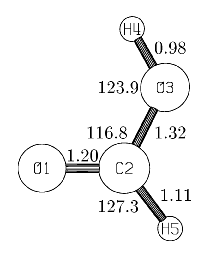
\includegraphics{pichcooh}
\end{center}
\caption{\label{hcooh} Data set for Formic acid}\index{Data! for formic acid}
\end{figure}

The geometry in this data-set can be understood as follows: Atom 1, an oxygen,
is at the origin of internal coordinate space, and has  coordinates (0,0,0).
Atom 2, a carbon, is positioned at coordinate  (1.20,0,0), that is, it is
related to the oxygen  by  a  bond-length  of  1.20 \AA ngstroms,  and to atom
3, an oxygen, by a bond-length of 1.32 \AA ngstroms. The O-C-O angle is 116.8
degrees.  The first hydrogen is  bonded  to  the hydroxyl  oxygen  and  the
second hydrogen is bonded to the carbon atom. The H-C-O-O dihedral angle is 180
degrees.
